% ----------------------------------------------------------------------
% Nobby compatible default settings.

% 11pt and 12pt fonts usually work but may exhibit errors in
% conjunction with the --scale option.
% 
% Use documentclasses other than 'article' at your own risk.
% ----------------------------------------------------------------------
\documentclass[10pt]{article}
\usepackage{amsmath, amsthm, amssymb}
\usepackage[latin1]{inputenc}
\usepackage{graphicx}

% Nobby will copy the title and author as comments into the HTML file.
\title{Nobby Demo}
\author{Oliver Nagy (olitheolix@gmail.com)}

% ----------------------------------------------------------------------
% Include- and define your own packages and macros here, set LaTeX
% counters and variables, etc.
% ----------------------------------------------------------------------
\usepackage{tikz}
\usetikzlibrary{calc, through, arrows}
\usepackage{subcaption}
\usepackage[pdftex,bookmarks=true, pdftitle={Nobby Demo},
pdfauthor={Oliver Nagy}, colorlinks=true,
citecolor=black, linkcolor=black]{hyperref}

% Custom macro.
\newcommand{\mvec}[1]{\mathbf{#1}}

% New theorem environment. If you define eg. '\newtheorem{foo}{Foo}',
% be sure to add 'foo' to 'config.counter_names'.
\newtheorem{theorem}{Theorem}

% ----------------------------------------------------------------------
% Do not (re)define macros, environments, counters, variables,
% etc. beyond this point.
% ----------------------------------------------------------------------
\begin{document}
\maketitle

\section{Outline}
\label{sec:one}
This file demonstrates some of the constructs Nobby can convert to
HTML. Nobby relies on properly formatted \LaTeX code to do its work
properly.

Here is Pythagoras' theorem in an \emph{align} environment:
\begin{align}
  \label{eq:pyth}
  z = \sqrt{x^2 + y^2}.
\end{align}
Here it is again as an inline formula: $z = \sqrt{x^2 + y^2}$.

Nobby automatically escapes the <> characters. It is therefore safe to
write <strong> or </strong> without accidentally inserting HTML tags.

Similarly, Nobby also translate quotes: ``text in quotes'' and
escaped \LaTeX symbols like ``\$'', ``\{``, ``\}'' and ``\%'' to
proper HTML, ie. without the leading backslash.


\subsection{More formatting}
You can, of course, \emph{emphasise} something.

Inline math expressions like $x=1$ or $e^{i\pi} + 1 = 0$ work fine.

Here is some plain text. {{This sentence is actually an SVG image.}}

The \texttt{\textbackslash{ldots}} command is often useful\ldots as is the
\texttt{typewriter font}, or a \textbf{bold} statement.

\subsection{Environments}
Nobby does not know about \LaTeX macros or environments. It converts
them to images unless a plugin exists for them. The following examples
demonstrate some of the default plugins.

\subsubsection{Itemize}
\begin{itemize}
\item Item 1
\item Item 2
\end{itemize}

\subsubsection{Enumerate}
\begin{enumerate}
\item Item 1
\item Item 2
\end{enumerate}

\subsubsection{Equation}
\begin{equation}
  \label{eq:rel}
  E = mc^2.
\end{equation}

\subsubsection{Theorem}
There is no default plugin for theorems -- the entire theorem below is
thus an image (compare the quality of this version with the
\href{http://en.wikipedia.org/wiki/Divergence_theorem}{original} on Wikipedia).
\begin{theorem}[Divergence Theorem]
  Suppose $\mathcal{V}$ is a subset of $\mathbb{R}^n$ (in the case of
  $n=3$, $\mathcal{V}$ represents a volume in 3D space) which is
  compact and has a piecewise smooth boundary $\mathcal{S}$ (also
  indicated with $\partial\mathcal{V} = \mathcal{S}$). If $F$ is a
  continuously differentiable vector field defined on a neighborhood
  of $\mathcal{V}$, then we have
  \begin{align}
    \iiint_{\mathcal{V}} \nabla \cdot F(\mvec{v})\; \textnormal{d}\mvec{v}
    = \oint_{\mathcal{S}} F(\mvec{s})\; \textnormal{d}\mvec{s}.
  \end{align}
\end{theorem}

Note that the equation number is wrong (it should be 3, not 2). The
reason for this inconsistency is that Nobby only takes a snapshot of
the \LaTeX counters at the start of any environment listed in
\texttt{config.counter\_dump\_envs}. Add the string ``theorem'' to
that list and run Nobby again to rectify the problem.

Nobby also converts \LaTeX comments to HTML. You cannot see those
comments because, well, they are comments, alright. To see them anyway
switch to the source code view in your browser.
% By the way, Nobby also converts LaTeX comments to HTML.

\section{References}
\label{sec:ref}
Nobby supports references via the standard \texttt{\textbackslash{href}}
command. This works for equations, sections, tables, figures, and
more.

For instance, here is a numbered reference to Pythagoras' theorem
(\ref{eq:pyth}) and Einstein's famous formula (\ref{eq:rel}).

You may also use the \texttt{\textbackslash{hyperref}} command to
create named links to reference the formulae of
\hyperref[eq:pyth]{Pythagoras} and \hyperref[eq:rel]{Einstein}.

Next are some examples of referenced sections.

\subsection{Sub-Section}
\label{ss:1}
This is sub-Section \ref{ss:1} inside Section \ref{sec:ref}.

\subsubsection{Sub-Sub-Section}
\label{sss:1}
This is sub-sub-Section \ref{sss:1} inside sub-Section \ref{ss:1} and
Section \ref{sec:ref}. The \texttt{\textbackslash{hyperref}} also
works. For instance, you can link to the \hyperref[sec:ref]{main section}.

\subsubsection*{Starred Sub-Sub-Section}
Nobby also supports starred sections.

\section{Figures and Tables}
Here is a floating table. Whereas  \LaTeX would put it at a visually
pleasing position, Nobby puts it right where it was defined.
\begin{table}
  \centering
  \begin{tabular}{c | c c c c}
    & $\frac{\pi}{6}$& $\frac{\pi}{4}$& $\frac{\pi}{2}$ & $\pi$\\[1mm]
    \hline
    \rule{0cm}{4mm}$\sin(\phi)$& $\frac{1}{2}$ & $\frac{1}{\sqrt{2}}$& $1$ & $0$\\
    \rule{0cm}{4mm}$\cos(\phi)$& $\frac{\sqrt{3}}{2}$ & $\frac{1}{\sqrt{2}}$& $0$&$-1$
  \end{tabular}
  \caption{Floating table}
\end{table}

A conventional figure environment that uses the
\texttt{\textbackslash{subcaption}} package. The code and figures for
the next example are from the
\href{http://en.wikibooks.org/wiki/LaTeX/Floats,_Figures_and_Captions}{Wikimedia}
on \LaTeX. Note that the image is a PNG (hence the coarser appearance)
because the inclusion of the three other images exceeds the image size
threshold (you can adjust it in Nobby's \texttt{config.py} file).\\
\begin{figure}
  \centering
  \begin{subfigure}[b]{0.3\textwidth}
    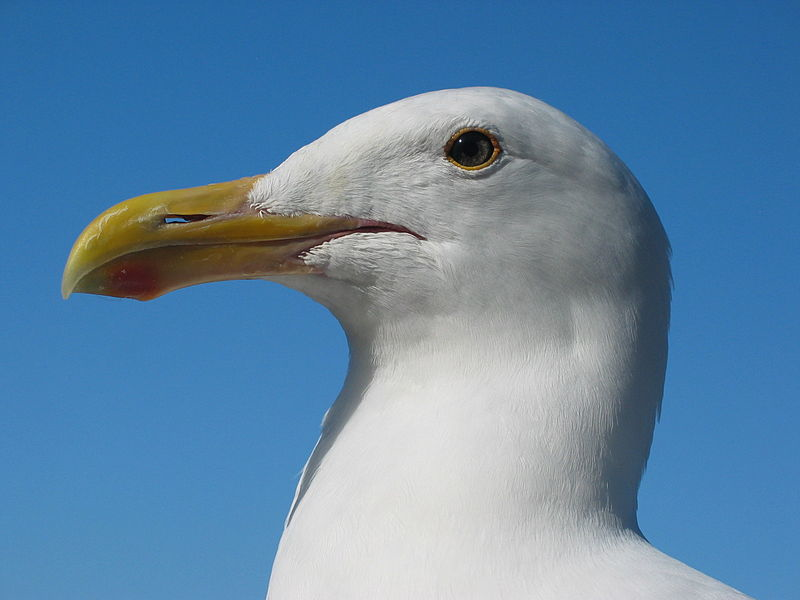
\includegraphics[width=\textwidth]{gull}
    \caption{A gull}
    \label{fig:gull}
  \end{subfigure}%
  ~ %add desired spacing between images, e. g. ~, \quad, \qquad etc.
  % (or a blank line to force the subfigure onto a new line)
  \begin{subfigure}[b]{0.3\textwidth}
    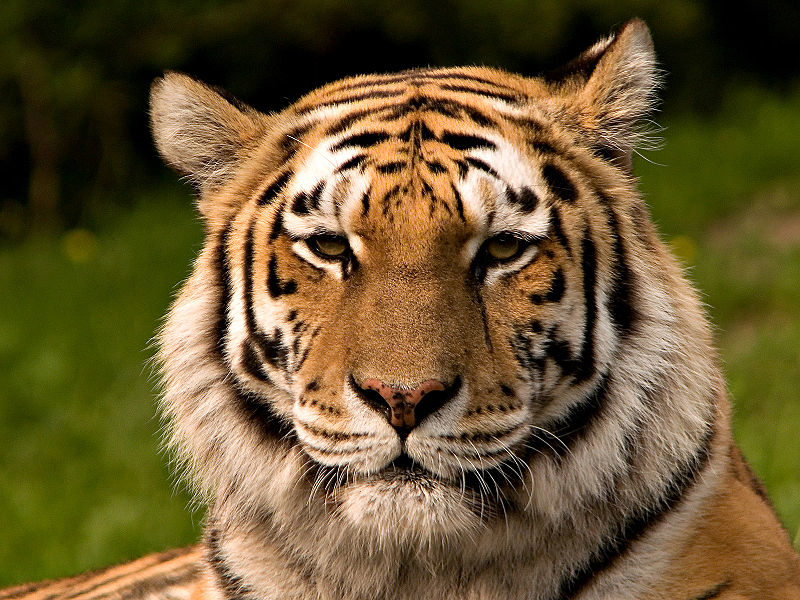
\includegraphics[width=\textwidth]{tiger}
    \caption{A tiger}
    \label{fig:tiger}
  \end{subfigure}
  ~ %add desired spacing between images, e. g. ~, \quad, \qquad etc.
  % (or a blank line to force the subfigure onto a new line)
  \begin{subfigure}[b]{0.3\textwidth}
    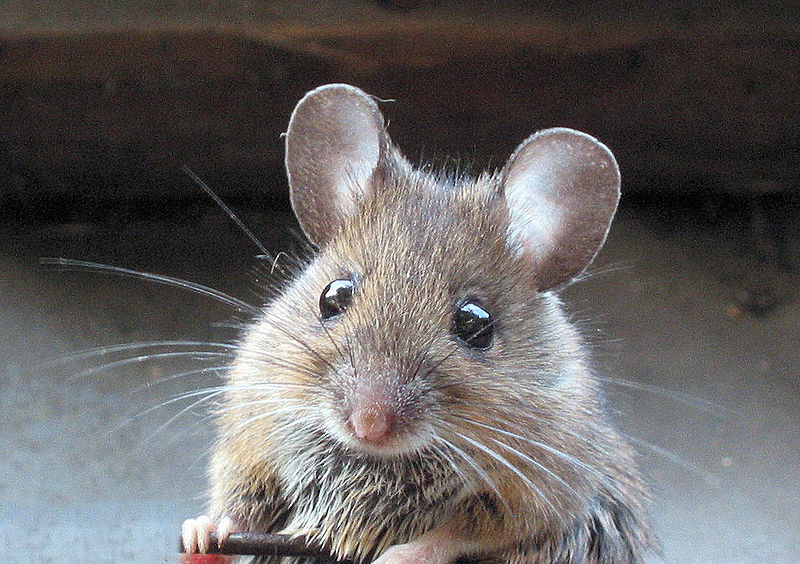
\includegraphics[width=\textwidth]{mouse}
    \caption{A mouse}
    \label{fig:mouse}
  \end{subfigure}
  \caption{Pictures of animals}\label{fig:animals}
\end{figure}

Here is Figure \ref{fig:gull} by itself. Note that the counter in the
figure caption increased (as expected).
\begin{figure}
  \centering
  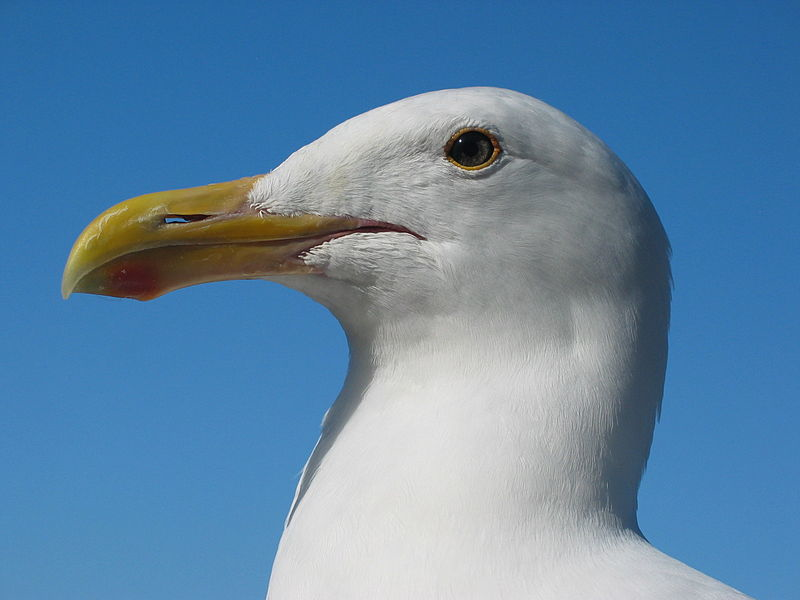
\includegraphics[width=\textwidth]{gull}
  \caption{The gull by itself.}
  \label{fig:gull_alone}
\end{figure}

\section{TikZ Image}
\emph{TikZ} is a popular \LaTeX package for technical drawings.
The following graph shows one of the
\href{http://www.texample.net/tikz/examples/j-curve}{publicly
  available} examples.
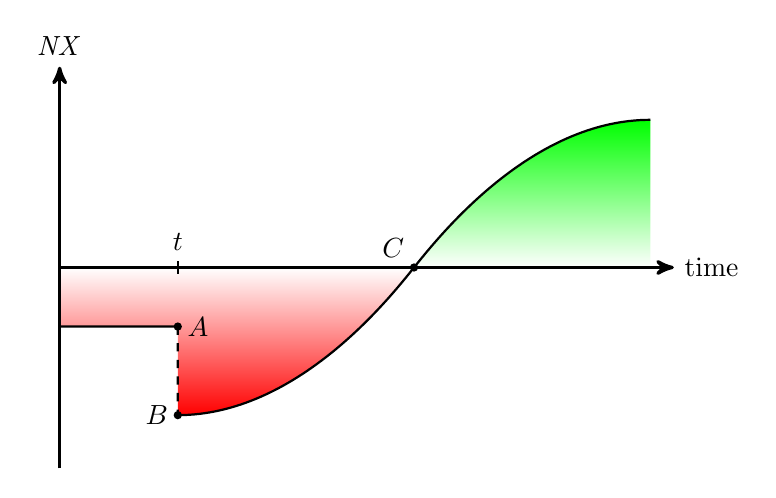
\begin{tikzpicture}[
        %We set the scale and define some styles
        scale=1.5,
        axis/.style={very thick, ->, >=stealth'},
        important line/.style={thick},
        dashed line/.style={dashed, thick},
        every node/.style={color=black,}
     ]
    % Important coordinates are defined
    \coordinate (beg_1) at (0,-.5);
    \coordinate (beg_2) at ($(beg_1)+(1,0)$);
    \coordinate (dev_1) at ($(beg_2)+(0,-.75)$);
    \coordinate (xint) at (3,0);
    \coordinate (end) at (5,1.25);

    %We make some nice shading to annotate different parts of the curve
    % Everything for x<0
    \begin{scope}
        \shade[top color=white, bottom color=red]
            ($(beg_2)+(0,.5)$) parabola bend (dev_1) (xint)
            (0,0) rectangle (beg_2);
    \end{scope}
    %  Everything for x>0
    \begin{scope}
        \shade[bottom color=white, top color=green]
            (xint) parabola bend (end) ($(end)+(0,-1.25)$);
    \end{scope}
    % axis
    \draw[axis] (0,0)  -- (5.2,0) node(xline)[right] {time};
    \draw[axis] (0,-1.7) -- (0,1.7) node(yline)[above] {$\mathit{NX}$};
    % J curve is drawn
    \draw[important line]
        (beg_1) -- (beg_2)
        (dev_1) parabola (xint)
        (xint) parabola[bend at end] (end);
    % coordinates are added
    \fill[black] (beg_2) circle (1pt) node[right] {$A$};
    \fill[black] (dev_1) circle (1pt) node[left] {$B$};
    \fill[black] (xint) circle (1pt) node[above left] {$C$};
    % The time of the devaluation is added
    \draw[dashed line] (beg_2) -- (dev_1);
    \draw[thick] (1,-1.5pt) -- (1,1.5pt) node[above] {$t$};
\end{tikzpicture}

The end.
\end{document}
